\chapter{Crecimiento de films de MgB$_2$ por sputtering}\label{C:sput}
\graphicspath{{figs/sput/}}
\chapterquote{La vida es como el Tetris, si no cometes errores es que estás desperdiciando oportunidades.}{Corolario del dicho anterior}
%%%%%%%%%%%%%%%%%%%%%%%%%%%%%%%%%%%%%%%%%%%%%%%%%%%%%%%%%%%%%%%%%%%%%%%%
En este capítulo se describen los avances que se han hecho en la búsqueda de crecer films de MgB$_{2}$ directamente por sputtering, esto es, se buscó crecer el material deseado en un sólo paso, tratando de evitar el proceso de recocido. La ventaja de este método, además de evitar el recocido, es que es altamente reproducible, limpio y es capaz de producir films con buena adherencia. La técnica consiste en impactar un blanco del material que se desea depositar (en este caso MgB$_{2}$) con iones de Ar que son acelerados por una diferencia de potencial $V$, de modo de arrancar partículas del mismo blanco para que luego se depositen sobre el sustrato. Como los iones transfieren su energía cinética a las partículas que son arrancadas del blanco, las mismas llegan al sustrato con energías que son del orden de los eV. De esta manera, los átomos que se depositan tienen energía suficiente como para explorar el sustrato de modo de ubicarse en lugar donde la energía de vínculo entre el sustrato y la partícula depositada es máxima. Como se dijo antes, esto implica la posibilidad de hacer films con elevada adherencia.

La ventaja de producir un film in situ, es decir, evitando el proceso de recocido, es que de esta forma se impide que el sustrato y el film reaccionen entre si, lo que contribuye a lograr una transición superconductora abrupta, tal como se requiere para la fabricación del detector.

El trabajo de crecimiento por sputtering fue realizado en el nuevo edificio de Nanociencia y Nanotecnología del Centro Atómico Bariloche, una obra que concluyó durante segundo semestre de la realización de este trabajo. En el mismo semestre se trasladaron las máquinas de sputtering y todos los equipos relacionados con los procesos de microfabricación, que estaban en el Laboratorio de Bajas Temperaturas del mismo Centro Atómico. Esto llevó a que el trabajo de crecimiento de films de MgB$_2$ por sputtering que se muestra en este capítulo, pudiera realizarse solamente en el tercer semestre de trabajo de esta tesis.
%\newpage
\section{Procedimiento}\label{S:sputproc}
Para el crecimiento de films por sputtering se utilizaron sustratos de zafiro (0001) que se pegaron a un calefactor con pintura de plata y un blanco de MgB$_2$ que fue adquirido comercialmente. Se eligió utilizar un sustrato de zafiro por las mismas razones mencionadas en el capítulo \ref{C:evap}. La realización de los depósitos se inició haciendo vacío con una bomba mecánica y encendiendo luego una turbomolecular, con la que se hizo vacío hasta llegar a una presión del orden de $10^{-6}$\,Torr. Luego se calentó el sustrato hasta la temperatura de crecimiento T$_{crec}$ deseada y se lo mantuvo en dicha temperatura por una hora, al mismo tiempo que se hacía circular Ar dentro de la cámara. Se llevó a cabo este procedimiento porque se notó que al calentar el sustrato la presión en la cámara se incrementaba, probablemente debido al desgase del sustrato y de la pintura de plata que se utilizó para pegar el mismo sustrato al calefactor. Una vez purgado el sistema se lograba una presión base para los depósitos de 1\~-\~3\,$\times$10$^{-6}$\,Torr. Durante la realización de este trabajo se variaron diferentes parámetros pertinentes al crecimiento de films, a saber, T$_{crec}$, presión de Ar y potencia aplicada al blanco.

La velocidad de crecimiento del film $v_{crec}$ es proporcional al número de iones Ar que impactan en el blanco y a un coeficiente $Y$ denominado sputtering yield, que indica cuántos átomos del blanco son arrancados cada vez que impacta un ion en el mismo. Ahora bien, el número de iones que impactan en el blanco es directamente proporcional a la corriente que circula por el mismo, mientras que el sputtering yield es una función no lineal de la energía con la que los iones colisionan con el material. Sin embargo, si la energía cinética $K$ de los iones al momento de la colisión es suficientemente baja, se observa experimentalmente que $Y$ es proporcional a la misma. Por otro lado, la energía cinética de los iones va a ser directamente proporcional a la tensión aplicada al blanco, a partir de lo cual se puede concluir que, si la tensión aplicada es lo suficientemente baja (menor a 10$^4$\,V), se tiene que $Y \ \varpropto \ K \varpropto \ V$. Juntando este resultado con el hecho de que el número de iones que impactan en el blanco es proporcional a la corriente $I$ se tiene que:
\begin{equation}
v_{crec} \ \varpropto \ I \ Y \ \varpropto \ I \ V \ = \ P
\label{eq:vcrec_2}
\end{equation}
\noindent
siendo $P$ la potencia aplicada al blanco. El equipo de sputtering utilizado en este trabajo permite controlar la potencia que se aplica al blanco, es decir, que permite controlar que la velocidad de crecimiento sea constante.
\nomenclature{$K$}{Energía cinética.}
\nomenclature{$P$}{Potencia eléctrica.}
\nomenclature{$Y$}{Sputtering yield.}
%\newpage

La temperatura del sustrato se controló con un calefactor y un controlador PID. La temperatura se midió con una termocupla que censaba la base del calefactor. Para estimar la diferencia de temperatura entre la termocupla y la superficie del sustrato se supuso que la termocupla está acoplada perfectamente a la base del sustrato. Pensando que el sistema llegó a un estacionario se estimó la diferencia de temperatura a partir de la expresión\cite{incropera}:
\begin{equation}
	\Delta T \ = \frac{d_s\,\dot{q}}{A_s\,\kappa} \ \sim \ 5\,\mathrm{ºC}
	\label{eq:conduccion}
\end{equation}
\noindent
En este caso $d_s$ es el espesor del sustrato ($\sim$ 0.05\,cm), $A_s$ es el área del mismo ($\sim$\,0.25\,cm$^{2}$) y $\kappa$ su conductividad térmica a 200\,ºC ($\sim$ 0.1\,W/(cm\,K))\cite{tablaconductividad}. Para estimar el flujo de calor $\dot{q}$ del calefactor hacia el sustrato se supuso el peor caso posible, en el que toda la potencia disipada va a parar al sustrato, lo que no es cierto.  Como el calefactor tenía una resistencia de 1,6\,$\Omega$ y por él circulaba una corriente de aproximadamente 2\,A, el flujo máximo de calor hacia el sustrato se estimó en 6,4\,W. Bajo las mismas suposiciones, y tomando como dato adicional el calor específico $c_p$ del zafiro a 200\,ºC ($\sim$ 1\,J/(g\,K))\cite{tablacalor} y su densidad $\delta$ (4\,g/cm$^{3}$)\cite{Ekin2006} se estimó el tiempo característico del sistema:
\begin{equation}
	\tau_{relaj} \ = \delta\,d_s^2\,\frac{c_p}{\kappa} \ \sim \ 0.1\,\mathrm{s}
	\label{eq:relajacion}
\end{equation}
\noindent
de donde se concluye que el sistema estaba completamente estabilizado antes de empezar a realizar el depósito.
\begin{table}[h!]
\centering
\begin{tabular}{|c||c|c|c|c|c|c|} \hline
Muestra	& Potencia/W & T$_{crec}$/ºC & p/mTorr & D/pulgadas & t/min & Espesor/nm \\ \hline \hline
BMB2S1B1 & 50 &	-	& 10 & 2,75	&  30 &	- \\
BMB2S2B1 & 50 &	-	& 10 & 2,75	&  45 &	580\,$\pm$\,20 \\
BMB2S3B1 & 50 & - & 10 & 2,75 &  90 & 1120\,$\pm$\,20 \\
BMB2S4B1 & 50 & - & 10 & 2,75 &  90 & 920\,$\pm$\,10 \\
BMB2S5B1 & 50 & - & 10 & 2,75 &  90 & - \\ \hline
BMB2S1B2 & 50 & 225 & 10 & 2,75 &  90 & - \\
BMB2S2B2 & 50 & 275 & 10 & 2,75 &  90 & - \\
BMB2S3B2 & 50 & 250 & 10 & 2,75 &  90 & - \\
BMB2S4B2 & 50 & 240 & 10 & 2,75 &  90 & - \\ \hline
BMB2S1B3 & 100 & 100 & 10 & 2,75 &  20 & 60\,$\pm$\,30 \\
BMB2S2B3 & 100 & T$_{amb}$ & 10 & 2,75 &  30 & 960\,$\pm$\,60 \\
BMB2S3B3 & 100 & 225 & 10 & 2,75 &  30 & 890\,$\pm$\,50 \\
BMB2S4B3 & 50 & 225 & 50 & 2,75 &  30 & 354\,$\pm$\,8 \\ 
BMB2S5B3 & 50 & 500 & 10 & 2,75 &  15 & 120\,$\pm$\,40 \\
BMB2S6B3 & 50 & 225 & 100 & 2,75 &  20 & 200\,$\pm$\,20 \\  
BMB2S7B3 & 100 & 225 & 100 & 2,75 &  22 & 540\,$\pm$\,20 \\ \hline
BMB2S1B4 & 100 & 225 & 50 & 2.75 & 6 & 190\,$\pm$\,20 \\ \hline
\end{tabular}
\caption{Resumen de los distintos parámetros explorados para realizar los depósitos de MgB$_2$.}
\label{tab:depositos}
\end{table}
%\newpage

En la tabla \ref{tab:depositos} se encuentran resumidos los depósitos realizados en el transcurso de esta tesis, junto con los respectivos parámetros relevantes. La medición de la distancia que se muestra en la tabla \ref{tab:depositos} es la que corresponde a la lectura indicada por un tornillo graduado que permitía regular la distancia entre el sustrato y el blanco. El valor de 2.75 pulgadas mostrado equivale aproximadamente a una distancia blanco - sustrato de 3\,cm. Para determinar el espesor de los films se midió la altura de un escalón generado en la muestra a partir de colocar pintura de plata en una parte del sustrato, que era removida luego de depositar la muestra. La medición del escalón se realizó utilizando el mismo perfilómetro de aguja de la sección \ref{S:evapcarac}, siguiendo el mismo procedimiento que el explicado en aquella sección.

La formación de films de MgB$_{2}$ requiere el cumplimiento simultáneo de dos condiciones: por un lado, se debe tener la proporción correcta de Mg y B en el film y además se debe lograr formar la estructura cristalina adecuada. Para lograr el cumplimiento de estas dos condiciones los pa\-rá\-me\-tros de crecimiento deben ser elegidos con cuidado. Por un lado, si se quiere formar la fase MgB$_{2}$ se necesita elevar la temperatura del sustrato\cite{Naito2004, Zhai1995, Xi2004}. Por otro lado, dado que el Mg es un elemento muy volátil, una temperatura demasiado grande lleva a que poco o nada del Mg se termine depositando, lo que resulta en deficiencia de Mg\cite{Xi2004}. Para solucionar este problema se puede incrementar la presión de Mg durante el cre\-ci\-mien\-to, cosa que se puede hacer incrementando la velocidad de depósito, esto es, la potencia aplicada al blanco. Esto puede resultar en una mala topografía y estructura cristalina. También se puede controlar la energía con la que los iones llegan al sustrato, ajustando la presión de Ar dentro de la cámara. La presión de Ar determina el camino libre medio de los iones que salen del blanco. A mayor presión de Ar, las partículas que salen del blanco sufren más colisiones, y por lo tanto llegan con menos energía al sustrato. En este caso las consecuencias de que los iones lleguen con más o menos energía son análogas a las que se pueden esperar si la temperatura es más elevada o más baja. Al llegar con más energía, las partículas tienen más capacidad de explorar la superficie y encontrar el lugar óptimo en donde depositarse, lo que resulta en una mejor adherencia y estructura cristalina.

Los films producidos fueron caracterizados en los tres aspectos relevantes para este trabajo: en primer lugar se caracterizó su estructura cristalina a partir de difracción de rayos X, en segundo se caracterizó su composición por medio de dos técnicas complementarias, retrodispersión de Rutherford (RBS) y emisión de rayos X característicos (EDX), y por último se caracterizó las propiedades superconductoras de los films a partir de mediciones de transporte y magnetización en un magnetómetro SQUID.
\nomenclature{$d_s$}{Espesor del sustrato.}
\nomenclature{$A_s$}{Área del sustrato.}
\nomenclature{$\dot{q}$}{Flujo de calor.}

\section{Caracterización de los films de MgB$_2$}\label{S:caract}
\subsection{Espesores y velocidad de crecimiento}\label{SS:espesor}
La medición de los espesores se hizo utilizando el mismo método que en la sección \ref{S:evapcarac}. En la figura \ref{fig:calibracion} se encuentran las curvas que muestran el espesor en función del tiempo de depósito para las dos potencias utilizadas. Se ajustaron rectas, forzando el paso por 0, a los valores experimentales obtenidos para tener una estimación de la velocidad de crecimiento de los films de MgB$_2$ sobre zafiro. El punto correspondiente a un tiempo de depósito de 20 min. y potencia aplicada de 100\,W fue descartado de los ajustes a partir de un análisis de bandas de confianza de 95\,\% y por lo tanto no influyó en el cálculo de la velocidad de crecimiento de los films.
\begin{figure}[tbh!]
 \begin{center}
    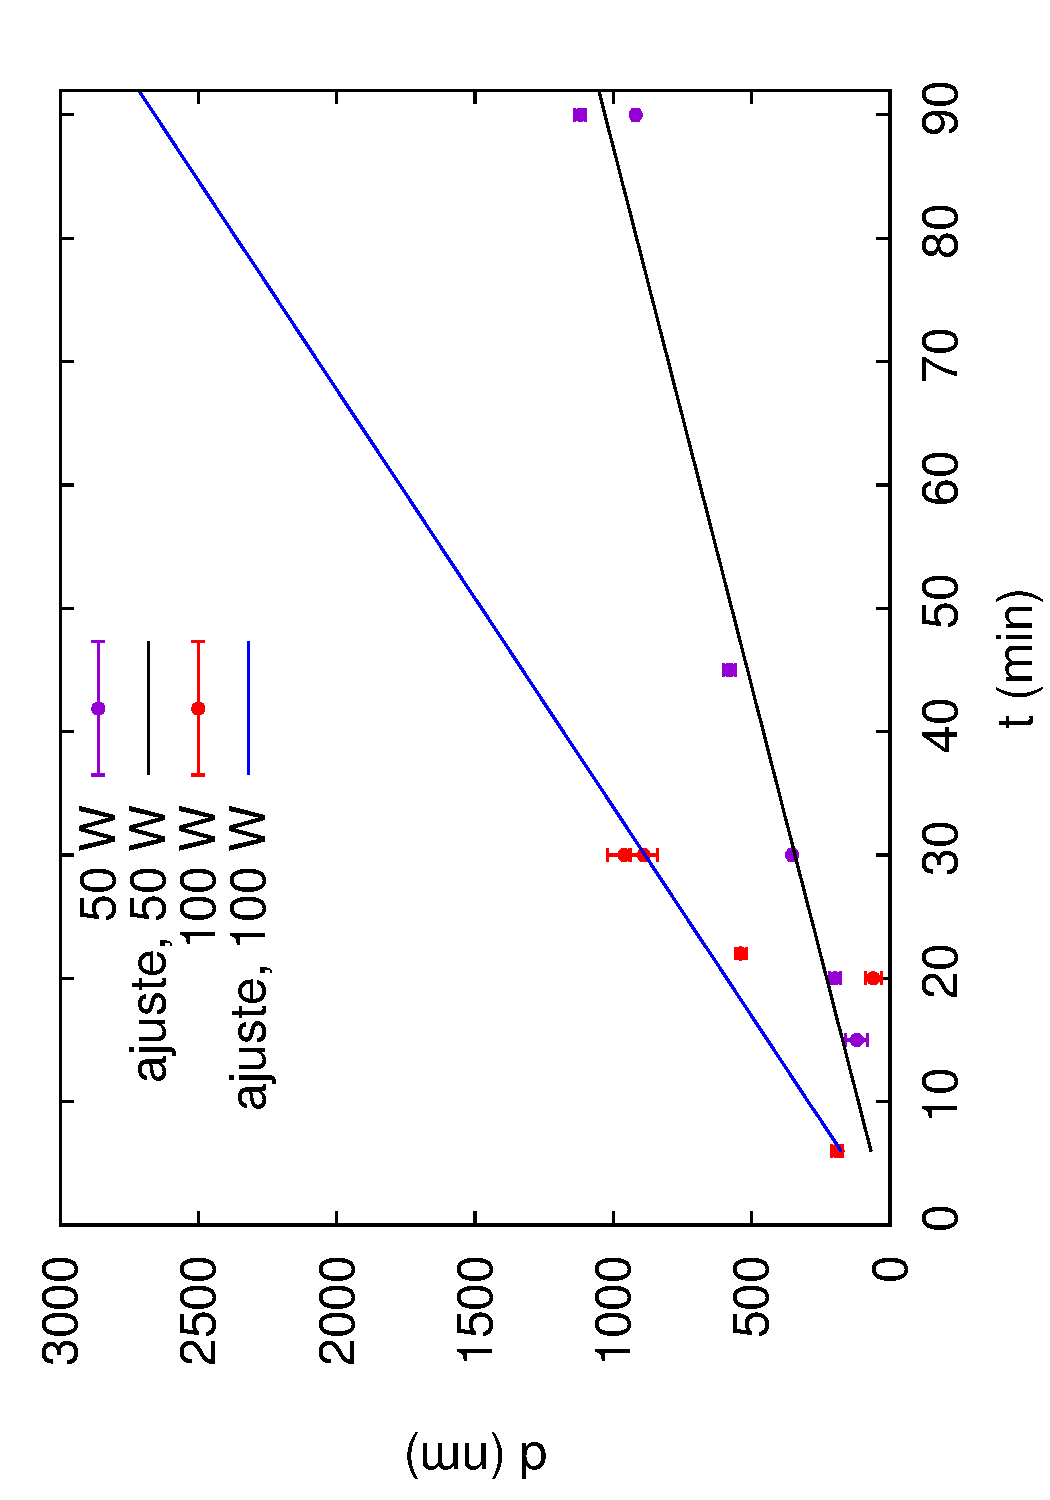
\includegraphics[width=0.5\columnwidth, angle=-90]{evst}
  \end{center}
\caption[Espesor en función del tiempo para los films de MgB$_2$ crecidos por sputtering.]{Espesor en función del tiempo para los films de MgB$_2$ crecidos. Se muestran las dos potencias utilizadas, junto con el ajuste correspondiente. Tomando como referencia dichos ajustes se estimó la velocidad de crecimiento de los films de MgB$_2$ en zafiro como $(12.9 \, \pm \, 0.5)$\,nm/s para una potencia aplicada de 50\,W y $(30 \, \pm \, 3)$\,nm/s para una potencia de 100\,W.}
\label{fig:calibracion}
\end{figure}

A partir de los resultados de los ajustes se estimó que la velocidad de crecimiento de los films de MgB$_2$ sobre zafiro, si la potencia es de 50\,W es $v_{crec, \, 50W}\, =\, (11.4 \, \pm \, 0.5)$\,nm/min, mientras que si la potencia aplicada es de 100\,W, se tiene $v_{crec,\, 100W}\, =\, (29 \, \pm \, 2)$\,nm/min. Los valores medidos se encuentran resumidos en la tabla \ref{tab:velocidadcrec}. Como puede verse, la velocidad de crecimiento a 100\,W es aproximadamente el doble de la velocidad de crecimiento a 50\,W, por lo que se puede concluir que en el régimen de presiones y potencias utilizados, la velocidad de depósito es aproximadamente lineal con la potencia aplicada, tal como se explicó anteriormente.
\begin{table}[h!]
\centering
\begin{tabular}{|c|c|c|} \hline
Potencia/W & Pendiente/(nm/min) & Ord. al origen (nm)\\ \hline
50 & $12.9\,\pm\,0.5$ & $-30\,\pm\,20$ \\ \hline
100 & $29\,\pm\,2$ & $0\,\pm\,50$ \\ \hline
\end{tabular}
\caption{Resultados de los ajustes realizados a los datos experimentales que se muestran en la Fig. \ref{fig:calibracion}.}
\label{tab:velocidadcrec}
\end{table}
\newpage
\subsection{Caracterización de la estructura cristalina por rayos X}\label{SS:rayos10}
La caracterización de muestras por medio del estudio de rayos X difractados es una de las prácticas más importantes a la hora de caracterizar materiales. La técnica consiste en incidir el material a estudiar con un haz de rayos X de longitud bien definida y medir la intensidad del haz reflejado en función del ángulo que forman la muestra y el haz incidente. Luego de una medición realizada en estas condiciones se obtiene un espectro que tiene picos a ángulos bien definidos que satisfacen la ley de Bragg:
\begin{equation}
  2 \ e \ \sin(\theta) \ = \ \lambda
  \label{eq:bragg}
\end{equation}
\noindent
siendo $\theta$ en ángulo formado entre la normal a la muestra y el detector de rayos X, $\lambda$ la longitud de onda incidente y $e$ es la separación entre la familia de planos cristalinos que cumplen la condición de Bragg. Los estudios de difracción de rayos X son muy útiles para determinar qué fases se encuentran un material y qué tipo de estructura cristalina poseen dichas fases.
\nomenclature{$e$}{Separación entre planos cristalinos.}
\nomenclature{$\theta$}{Ángulo formado entre la normal a un plano y la dirección de propagación de la radiación incidente/saliente.}

En el caso de las muestras que se desean estudiar en este trabajo aparecen dos complicaciones que vale la pena mencionar. La primera es que el bajo número atómico $Z$ del boro hace que sea muy difícil de detectar fases de boro puro en un espectro de rayos X, ya que la intensidad de los picos en un espectro de rayos X también se encuentra limitada por la sección eficaz entre el haz incidente y los átomos presentes en la muestra, que decrece como $Z^2$. El segundo factor a tener en cuenta es el siguiente: se puede ver que la integral de un pico de Bragg es proporcional al número de átomos presentes en los planos cristalinos que cumplen la condición \ref{eq:bragg}, mientras que el ancho del pico es inversamente proporcional a ese número. Esto implica que si la muestra es infinita los picos de Bragg del espectro de rayos X se aproximan a la función delta de Dirac. Sin embargo, en este trabajo se intenta caracterizar un film, por lo que, incluso si el mismo es un monocristal, es difícil que  logre satisfacer la condición de muestra infinita, con el resultado de que los picos de Bragg se vuelvan más anchos y de menor altura, si es que llegan a ser observados.

En la Fig. \ref{fig:rayos10} se muestran algunos de los espectros de difracción de rayos X para diferentes muestras, que corresponden a un barrido en la temperatura de crecimiento $T_{crec}$ de 225\,$^{\circ}$C a 275\,$^{\circ}$C (muestras BMB2S1B2 a BMB2S3B2) a 10\,mTorr y 50\,W; y una muestra en la que se incrementó la presión de Ar para el crecimiento (BMB2S6B3), mientras que la potencia fue de 50\,W y $T_{crec}\,=\,225$\,$^{\circ}$C.

Los dos picos de mayor intensidad que se encuentran señalados corresponden al sustrato de zafiro (0001) sobre el que se crecieron las muestras. Los picos más pequeños que se pueden ver antes del correspondiente a la familia de planos (0006), son debidos a la difracción de la radiación $K_{\beta}$ del Cu y a la L del W. Los picos correspondientes a la línea $K_{\beta}$ se pueden observar porque el monocromador que usa el equipo de rayos X no es perfecto, mientras que los picos debidos a la radiación de la capa L del W aparecen porque a lo largo de los años de uso del equipo, algo de W se fue depositando sobre la fuente de Cu. De esta forma, el W que se encuentra depositado es excitado junto al Cu, de modo que también emite radiación X que tiene una energía un poco diferente a la radiación X emitida por el Cu. 
\begin{figure}[tbh!]
 \begin{center}
    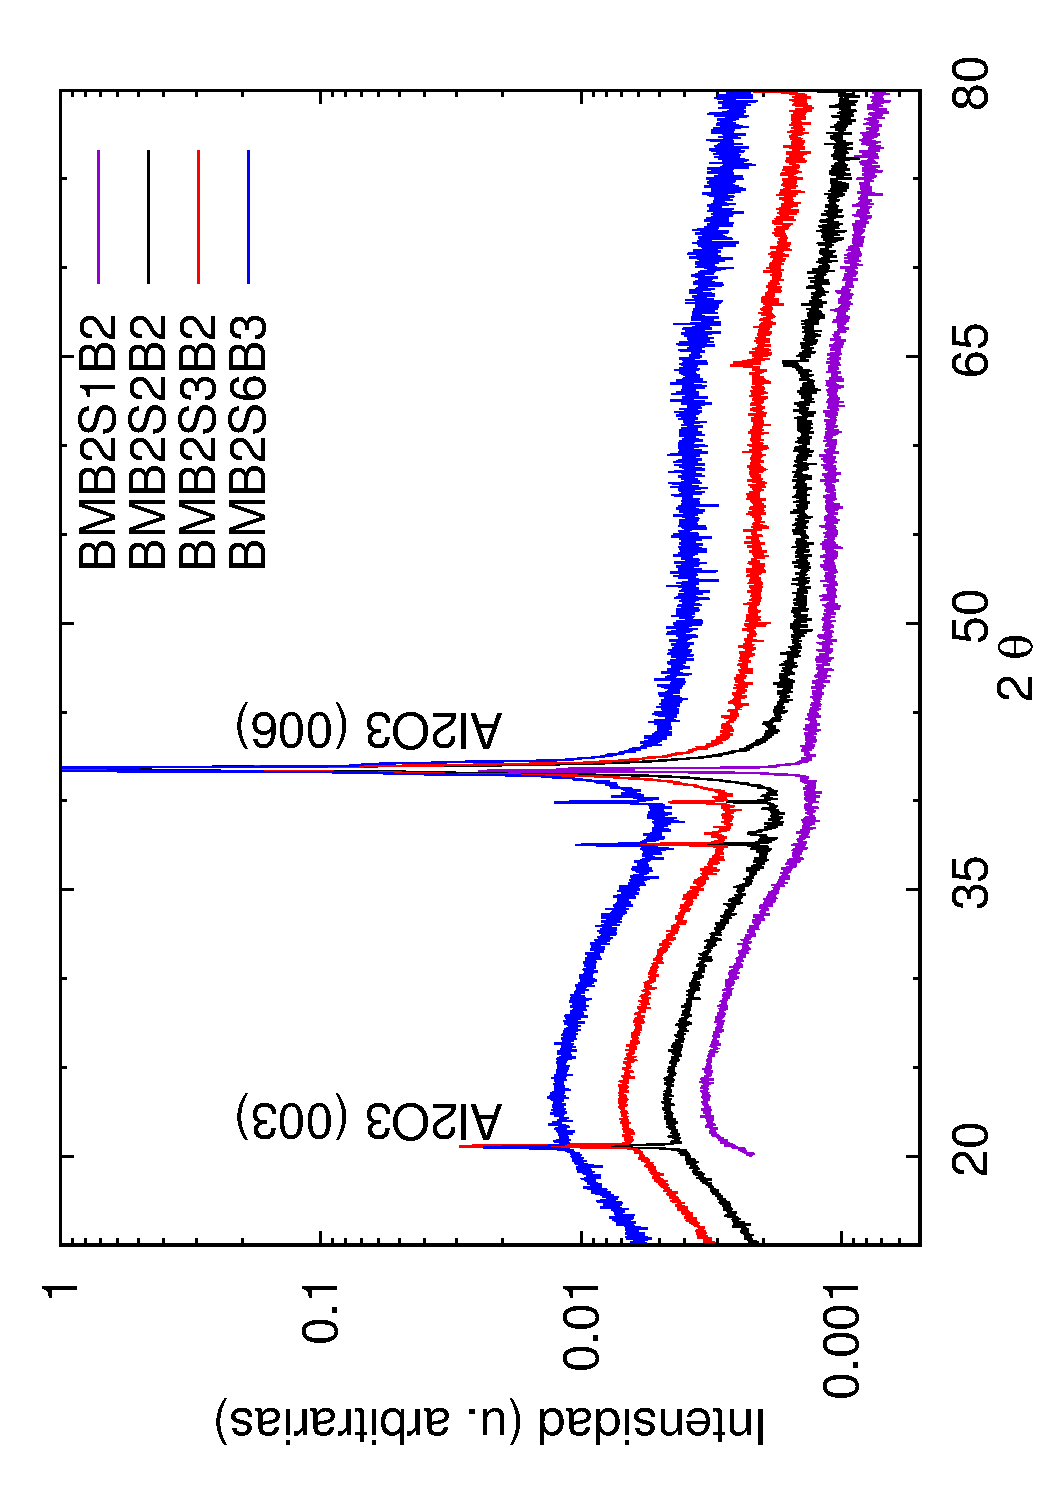
\includegraphics[width=0.5\columnwidth, angle=-90]{rayos10}
  \end{center}
  \caption[Espectro de difracción de rayos X para alguna de las muestras depositadas por sputterong.]{Espectro de difracción de rayos X para alguna de las muestras depositadas. Todos los picos observados corresponden a diferentes reflexiones del sustrato de zafiro (0001). Por otro lado puede observarse un pico muy ancho con un máximo alrededor de los 23\,$^{\circ}$. Esto se corresponde con el parámetro de red promedio del Mg policristalino.}
\label{fig:rayos10}
\end{figure}

Lo explicado en el párrafo anterior implica que todos los picos observados co\-rres\-pon\-den al sustrato de zafiro y que no se pueden apreciar picos correspondientes al MgB$_{2}$, y tampoco se pueden ver picos correspondientes a Mg o a B puros. A partir de éstos resultados pueden extraerse dos conclusiones: la primera es que se haya formado un film de MgB$_{2}$ con mala cristalinidad, o que no se haya formado la fase de MgB$_{2}$. Para verificar cuál de las dos hipótesis era la correcta, se realizaron análisis de la composición de los films y también se estudiaron las propiedades magnéticas y de transporte de los mismos. En las secciones siguientes se muestran los resultados de estos estudios.
\subsection{Caracterización de la composición por EDX}\label{SS:EDX}
La espectroscopia por rayos X característicos es una técnica ampliamente utilizada cuando se busca determinar la composición de un compuesto, y aunque no permite determinar la forma en que los elementos de un material se encuentran combinados, sí permite determinar con excelente precisión la proporción en que se encuentran dichos elementos. La técnica consiste en bombardear la muestra cuya composición se desea determinar con electrones que tienen la energía suficiente como para excitar a los electrones presentes en las primeras capas atómicas de los átomos presentes en la muestra. Posteriormente, los electrones del átomo se desexcitan emitiendo fotones que tienen una energía que es característica del átomo estudiado. A partir de colectar de estos fotones característicos se pueden construir histogramas como se muestra en la Fig. \ref{fig:SEM}, en el que se cuenta la cantidad de fotones que tienen una energía determinada, para un rango amplio de energías. El análisis de los picos observados permite identificar los elementos presentes en la muestra, así como la proporción de los mismos. Por razones parecidas a las que fueron comentadas en la sección anterior, el análisis por EDX se ve limitado para elementos livianos, siendo el B y el C  los elementos más livianos detectables por esta técnica.

En la Fig. \ref{fig:SEM} se muestran los espectros de intensidad emitida de rayos X característicos para dos de las muestras crecidas y para una pastilla de MgB$_{2}$ patrón hecha con polvo obtenido comercialmente. Dado que no se puede determinar directamente la composición de los films a partir de los métodos estándar que existen para el estudio de rayos X característicos, el método que se implementó para estimar la composición de los films fue el siguiente: del espectro obtenido para la muestra patrón, se calcula el cociente de las integrales de los picos correspondientes al B y al Mg ($Int_{B}$, $Int_{Mg}$, respectivamente). El cociente $Int_{B}/Int_{Mg}$ no tiene por qué se igual a 2. Esto es debido a que no se está haciendo la corrección de intensidades por número atómico, por absorción y por fluorescencia. Además, el hecho de que los rayos X característicos del B se encuentren en el borde de eficiencia del detector de rayos X también puede influir en que el número de cuentas que haya para los picos de B y Mg no sea proporcional a la cantidad de esos elementos en la muestra.
\begin{figure}[tbh!]
 \begin{center}
    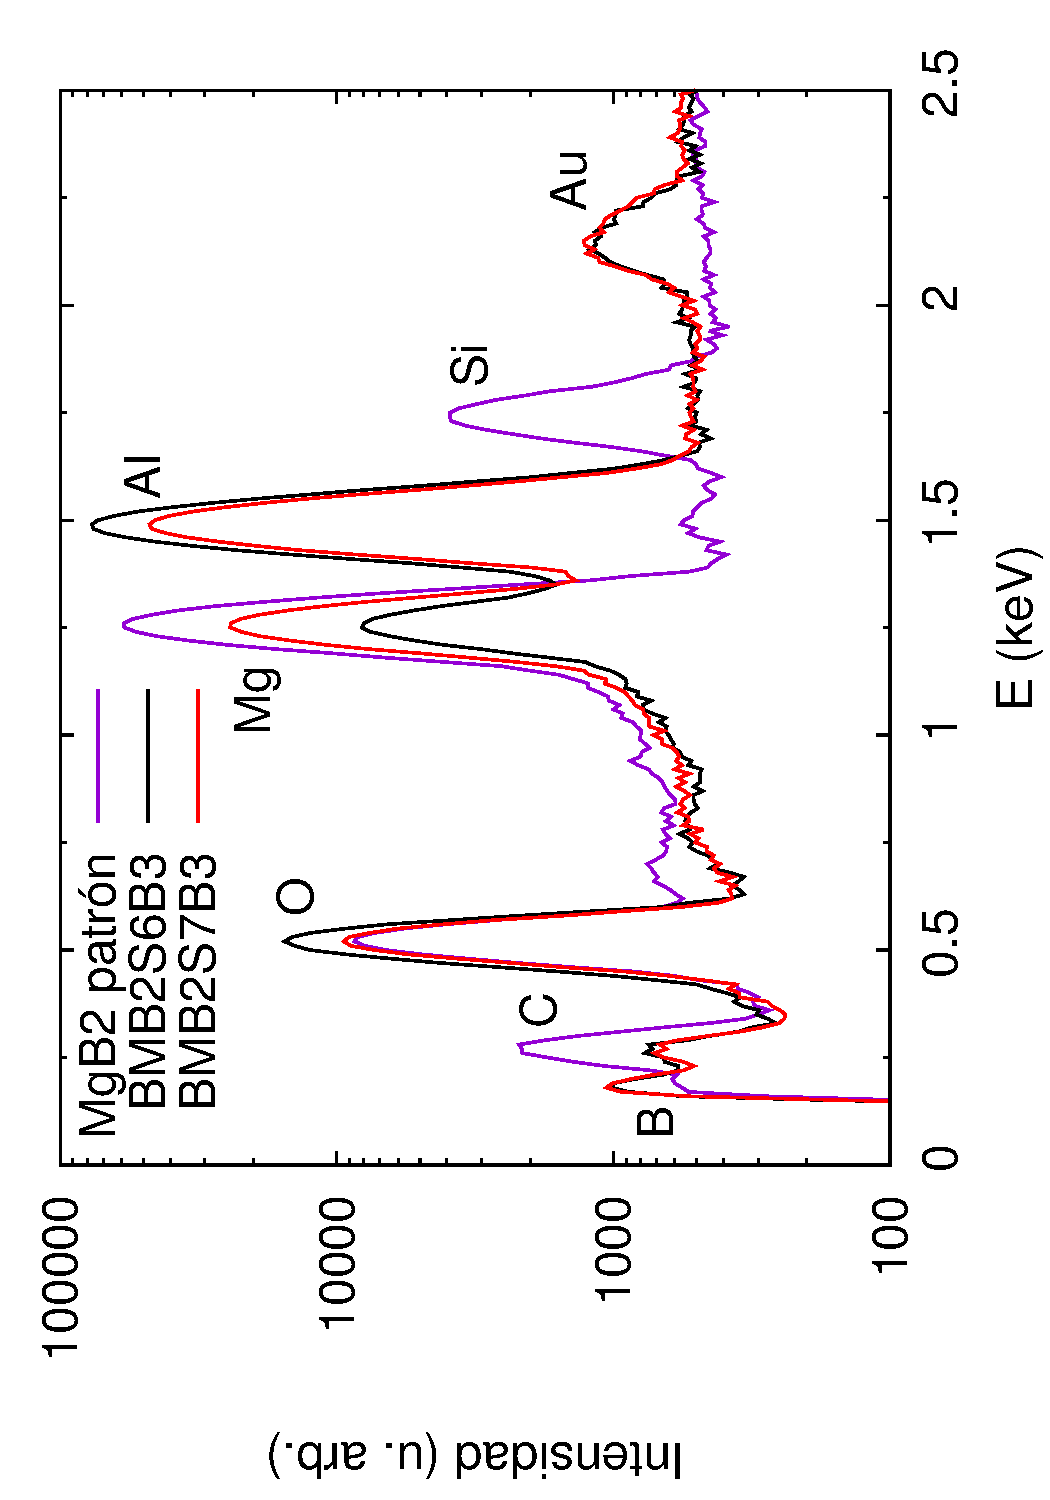
\includegraphics[width=0.55\textwidth,angle=-90]{SEM}
  \end{center}
  \caption[Espectro de la intensidad emitida de rayos X característicos para una muestra de MgB$_{2}$ patrón y para algunas de las muestras crecidas.]{Espectro de la intensidad emitida de rayos X característicos para una muestra de MgB$_{2}$ patrón y para algunas de las muestras crecidas. A partir de la comparación de las alturas relativas de los picos en el patrón se estimó la composición de los films crecidos.}
\label{fig:SEM}
\end{figure}

Una vez calculado el cociente ($Int_{B}/Int_{Mg}$)$_{bulk}$, al mismo se le asigna el valor 2, esto es, se define una constante $\varepsilon$ tal que:
\begin{equation}
  \varepsilon \ \left(\frac{Int_{B}}{Int_{Mg}}\right)_{bulk} \ = \ 2
  \label{eq:patron}
\end{equation}
%\newpage

Hecho esto, se realiza el cociente de la integral de los picos para las muestras cuya composición se desea estimar utilizando la misma constante de proporcionalidad $\varepsilon$:
\begin{equation}
  \varepsilon \ \left( \frac{Int_{B}}{Int_{Mg}} \right)_{film} \ = \ x
  \label{eq:film}
\end{equation}
\noindent
donde $x$ es la composición estimada del film. El cálculo de las áreas se hizo realizando un ajuste con una gaussiana a cada pico y luego integrando la función ajustada, sustrayendo una línea base que era una parábola. En los casos en que el pico de interés se superponía con el de otro elemento (por ejemplo, el B y el C, o el Mg y el Al) la línea de base consistió además en una gaussiana del pico vecino. Los centros de las gaussianas se mantenían fijos y eran tomados a partir de los datos de las líneas de emisión de cada elemento. En la Fig. \ref{fig:fiteos} se muestra un ejemplo del resultado de esta operación para uno de los films estudiados.
 \begin{figure}[tbh!]
   \begin{center}
	 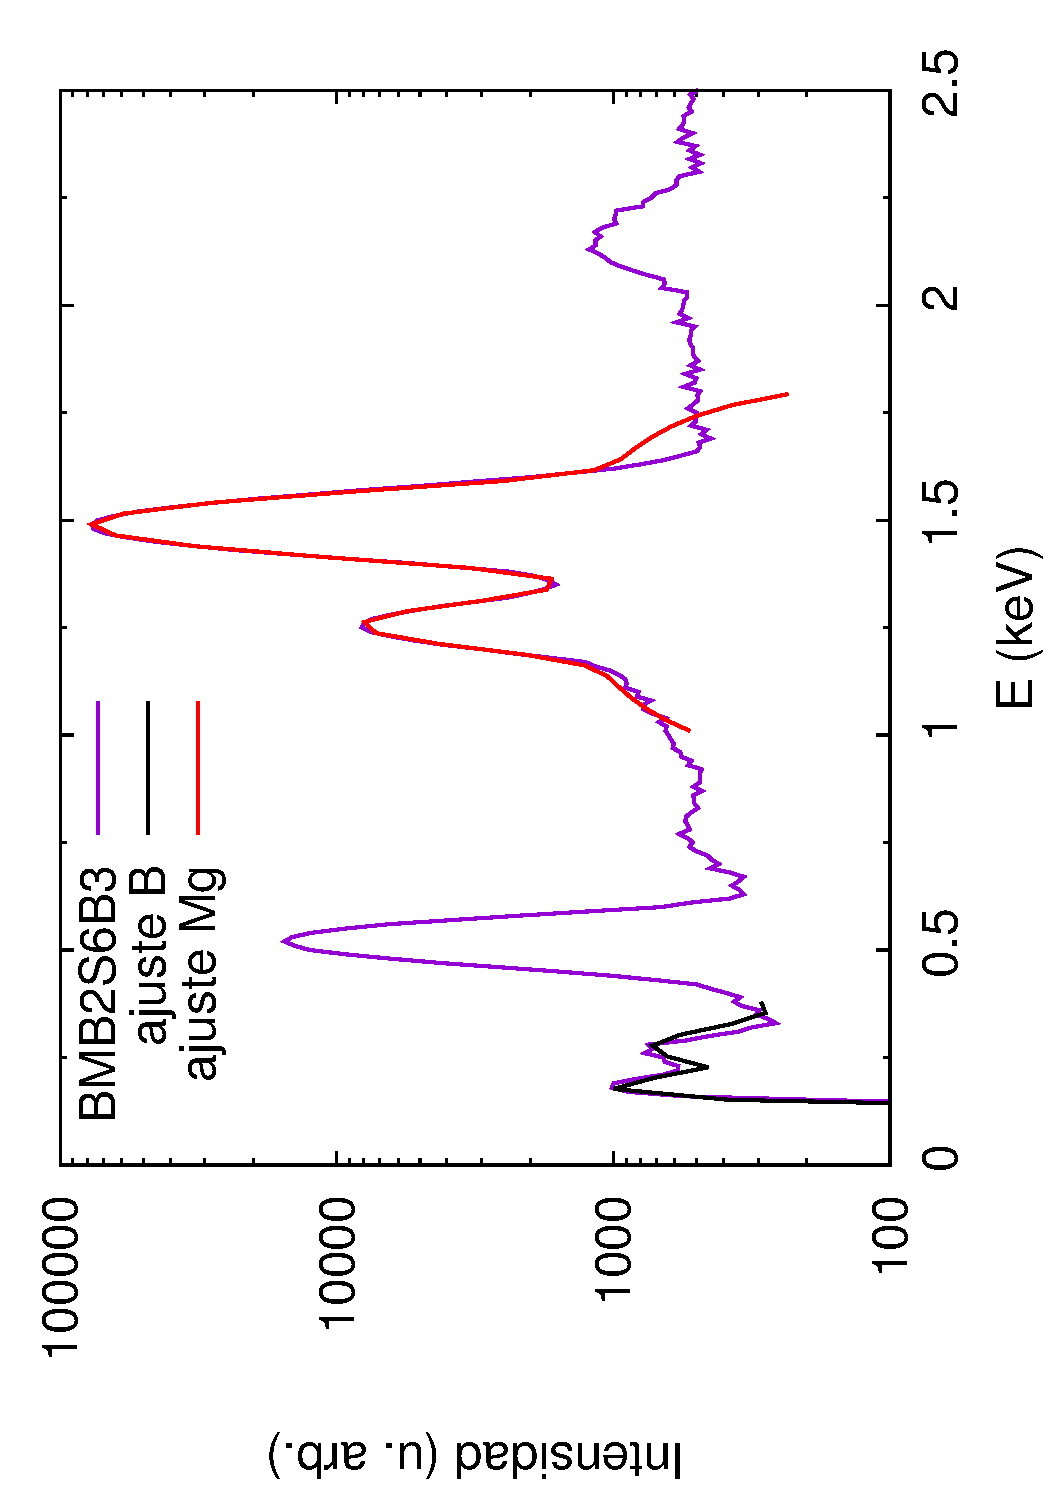
\includegraphics[width=0.55\textwidth, angle=-90]{fiteo}
   \end{center}
   \caption[Ejemplo del procedimiento empleado para estimar la composición de los films.]{Ejemplo del procedimiento empleado para estimar la composición de los films. Se ajustó una gaussiana al pico cuya área se deseaba estimar. Además se sumó una línea de base que consisitió en una parábola más una gaussiana asociada al pico vecino. Una vez sustraída la línea de base se calculó la integral de la gaussiana ajustada. A partir de la comparación de los cocientes de las integrales de los picos de B y Mg de los films con el patrón se estimó la composición de las muestras crecidas.}
   \label{fig:fiteos}
 \end{figure}

 A partir de los ajustes y cálculos realizados se estimó que la constante de proporcionalidad tiene el valor $\varepsilon\,=\,300\,\pm\,50$. Con $\varepsilon$ así calculado se construyó la tabla \ref{tab:composicionSEM}, en la que se compara la proporción B/Mg para las diferentes muestras estudiadas, junto con los parámetros de crecimiento relevantes que fueron modificados.

En las las tablas \ref{tab:depositos} y \ref{tab:composicionSEM} puede verse que la muestra BMB2S6B3 fue crecida en las mismas condiciones que la muestra BMB2S7B3, excepto que en la segunda la potencia aplicada al blanco era de 100\,W en vez de 50\,W. A partir de esto se puede suponer que un incremento en la potencia aplicada mejora la proporción B/Mg del film. Esto puede deberse a dos razones: la primera es que incrementar la velocidad de depósito implique de alguna forma un incremento en la presión de Mg en la proximidad del film, lo que produciría que deposite más Mg y por ende que aumente la proporción del mismo. La otra es que al incrementar la velocidad de depósito, es posible que el Mg quede ``atrapado'' por las demás partículas que están llegando del blanco y no tenga tiempo de evaporarse nuevamente.
 \begin{table}[h!]
  \centering
  \begin{tabular}{|c|c|c|c|}\hline
	Muestra	& Potencia/W & p/mTorr & Proporción B/Mg\ \\ \hline
	Patrón & - & - & 2 \\
	BMB2S6B3 & 50 & 100 & 27 $\pm$ 5 \\
	BMB2S7B3 & 100 & 100 & 8 $\pm$ 2 \\ 
	BMB2S1B4 & 100 & 50 & 28 $\pm$ 10 \\
	BMB2S3B3 & 100 & 10 & 14 $\pm$ 2 \\ \hline
  \end{tabular}
  \caption[Proporción B/Mg para las muestras estudiadas por EDX.]{Proporción B/Mg para las muestras estudiadas por EDX. Se muestran además los parámetros de crecimiento que cambiaron entre las diferentes muestras. En todos los casos la temperatura de crecimiento era 225\,$^{\circ}$C y la altura de crecimiento era 2,75, de acuerdo a lo indicado en la sección \ref{S:sputproc}. La única diferencia entre BMB2S6B3 Y BMB2S7B3 es que la primera fue crecida con una potencia aplicada de 50\,W mientras que la segunda lo fue con 100\,W. Las últimas tres muestras fueron crecidas con una potencia de 100\,W, pero con presión de Ar de 100\,mTorr, 50\,mTorr, 10\,mTorr, respectivamente.}
  \label{tab:composicionSEM}
\end{table}
%\newpage 
\nomenclature{$Int_{E}$}{Integral del pico correspondiente al elemento $E$, en un espectro de EDX.}
%\begin{figure}[tbh!]
%  \begin{center}
% 	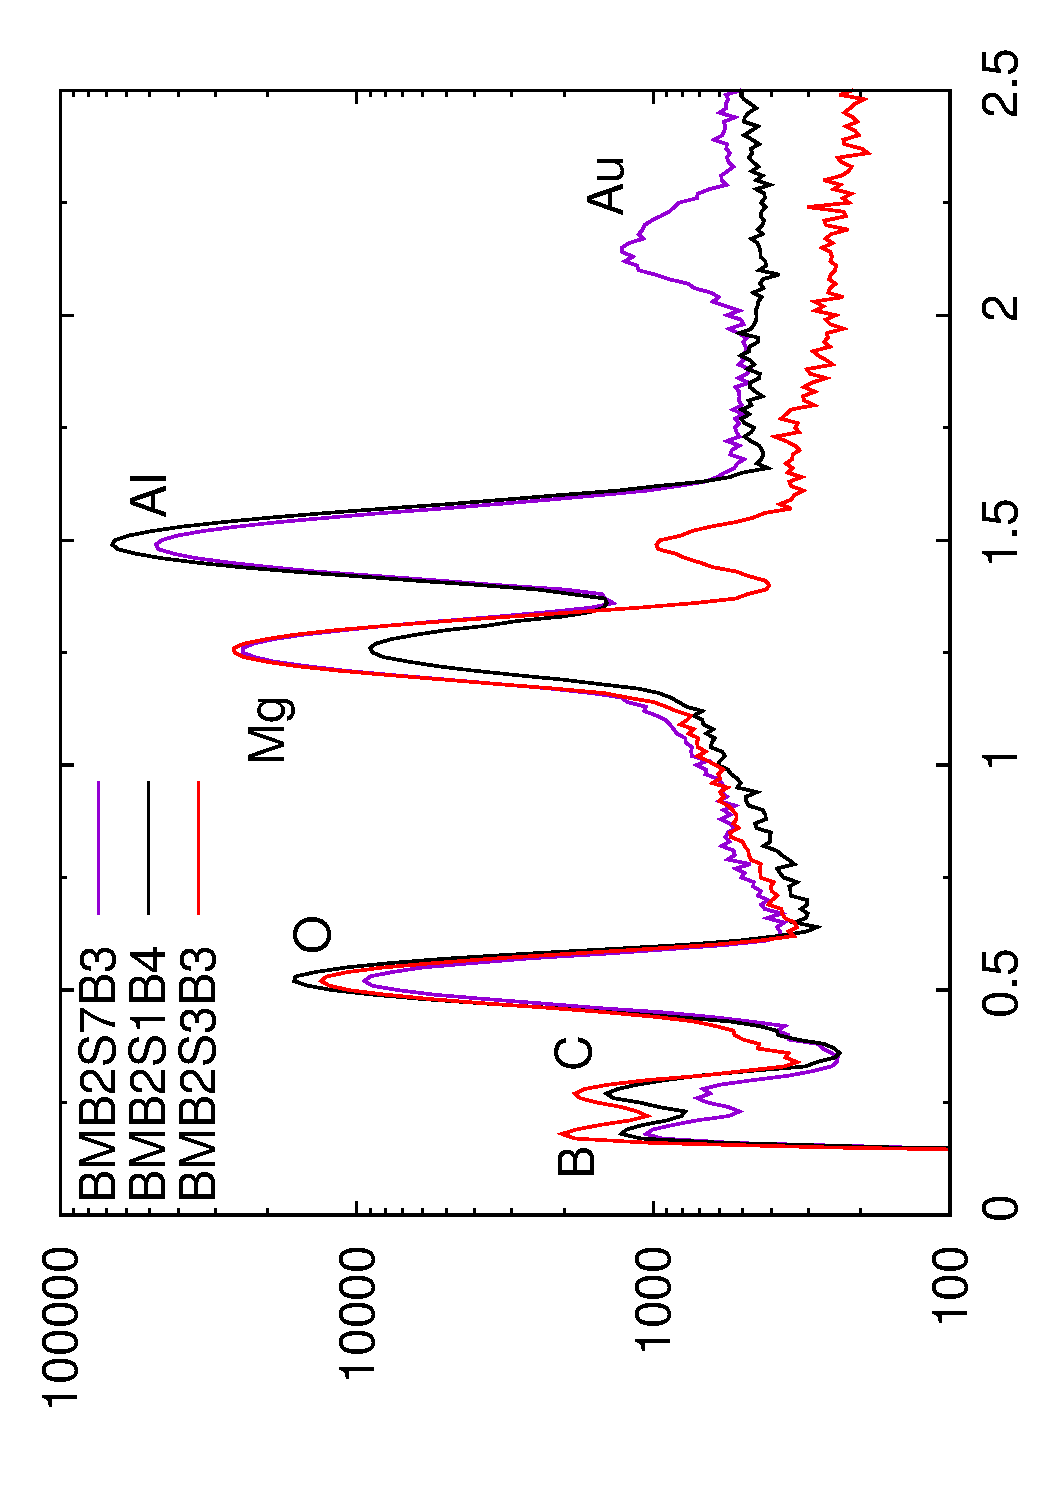
\includegraphics[width=0.55\textwidth, angle=-90]{SEM_cascada}
%  \end{center}
%  \caption{}
%  \label{fig:SEMcascada}
%\end{figure}

También se estudió el efecto que tiene la presión de Ar en la cámara en la composición final. En la tabla \ref{tab:composicionSEM} se muestra la proporción B/Mg de tres muestras crecidas en las mismas condiciones de temperatura y potencia, pero con diferente presión. Como se explicó al principio del capítulo, la presión de Ar en la cámara regula el camino libre medio de las partículas que salen del blanco, es decir, la cantidad de colisiones que sufren estas partículas antes de llegar al sustrato. De esta forma se puede controlar la energía cinética que tienen las mismas al momento de depositarse en el sustrato, lo que influye en la topografía del film, su adherencia con el sustrato y la estructura cristalina que se pueda formar.
 \begin{figure}[tbh!]
   \begin{center}
	 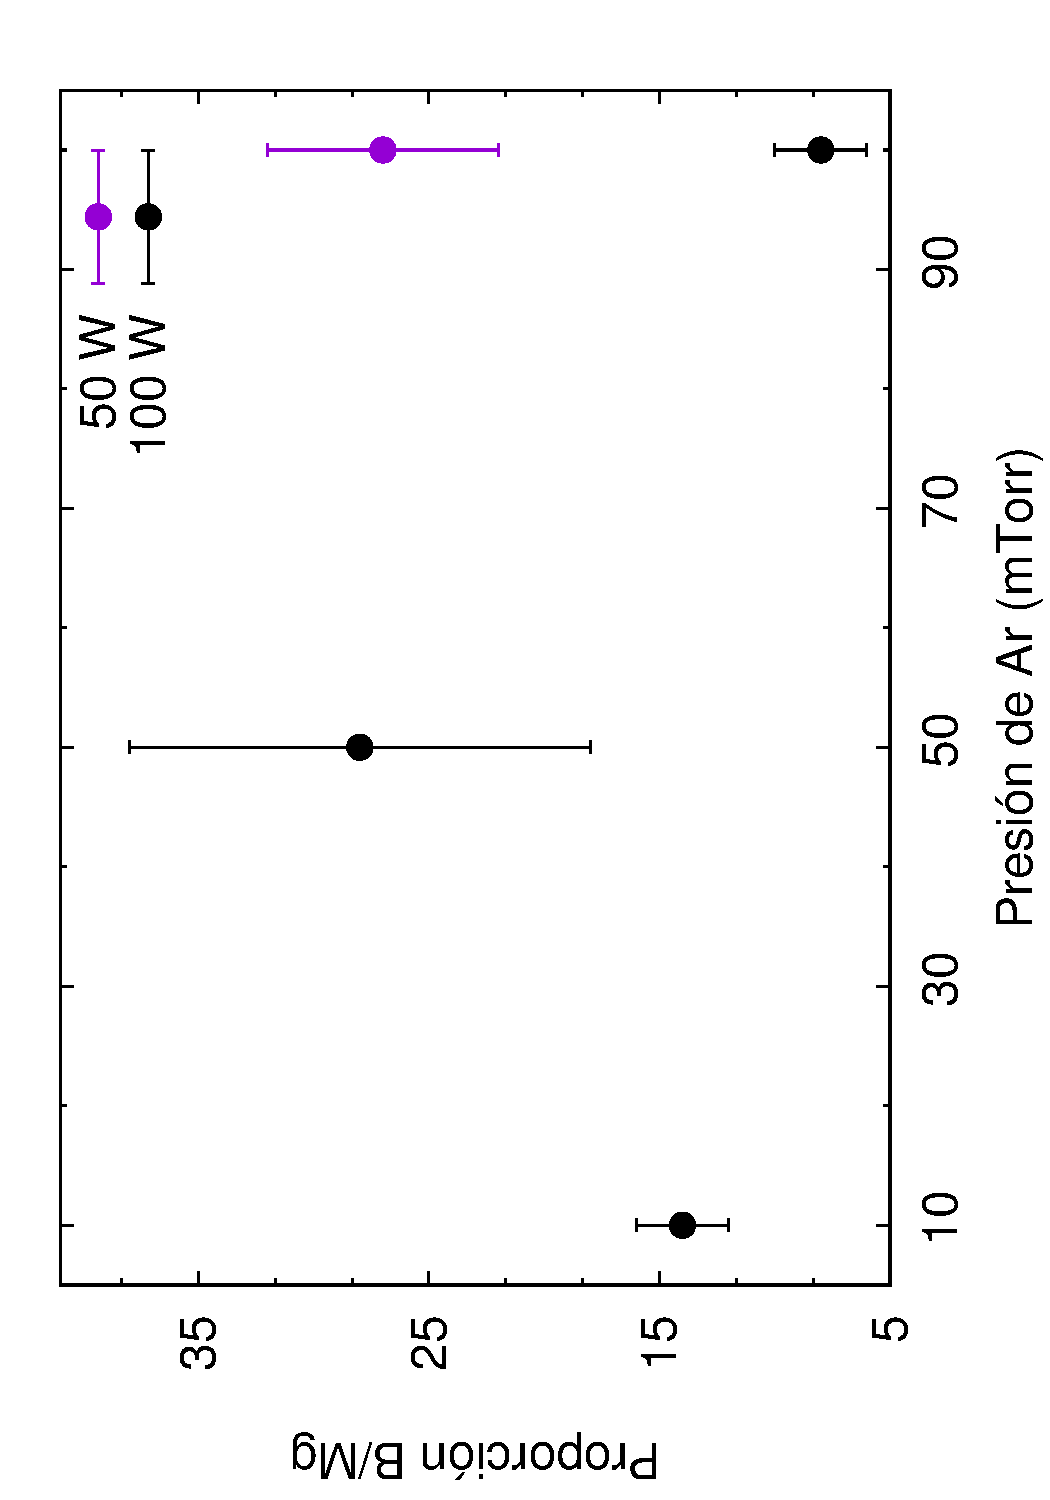
\includegraphics[width=0.55\textwidth, angle=-90]{xvsp}
   \end{center}
   \caption[Proporción B/Mg para films crecidos con diferente presión de Ar en la cámara de sputtering.]{Proporción B/Mg para films crecidos con diferente presión de Ar en la cámara de sputtering. También se muestra una medición en la que el parámetro variado fue la potencia aplicada al blanco. Puede verse que mientras que la potencia tiene un claro efecto positivo en la composición del film, el efecto de la presión no es del todo claro.}
   \label{fig:xvsp}
 \end{figure}
\newpage

 Al analizar el comportamiento de la proporción B/Mg con la potencia puede apreciarse que disminuye claramente al aumentar la potencia que se aplica al blanco, es decir, al aumentar la velocidad de crecimiento. En el gráfico se muestran barras de error que corresponden a una desviación de 1 $\sigma$, pero los valores se encuentran separados incluso si se considera una desviación de 2 $\sigma$, lo que valida la conclusión de que al incrementarse la velocidad de crecimiento, la proporción B/Mg se aproxima a la correcta. A partir de esto se podría plantear la propuesta de incrementar más aún la potencia aplicada al blanco, en busca de lograr la proporción B/Mg deseada. Sin embargo, esto no es posible ya que una potencia mayor podría llevar a romper el blanco. A partir de este inconveniente fue que se planteó estudiar el efecto que tiene la presión de Ar en la proporción B/Mg, resultando que ambas variables están relacionadas en forma no monótona. Esto es lo que podría interpretarse si se considera una desviación
%\newpage
\noindent
 de 1 $\sigma$ en la Fig. \ref{fig:xvsp}, pero si se considera la desviación de 2 $\sigma$ alrededor de los valores observados, la conclusión es que no existe una dependencia clara entre la proporción B/Mg y la presión de Ar en la cámara.
\subsection{Caracterización de la composición por RBS}\label{SS:RBS}
El estudio de la composición por RBS consiste en bombardear el film con iones que tienen una energía conocida y estudiar el espectro de energía con que salen las partículas después de la colisión con la muestra. Como proyectil de prueba se suelen utilizar iones de H o de He, en función de la masa de los átomos presentes en la muestra. Como los iones que están presentes en la muestra son livianos, el espectro de energía producido resulta ser bastante sensible si los elementos presentes en la muestra tienen $Z$ pequeño, ya que en ese caso la transferencia de energía es máxima. En este sentido la espectroscopia por RBS puede considerarse la contraparte de la técnica EDX. La composición del material puede estimarse proponiendo un modelo de capas del material y realizando un ajuste en el que los parámetros libres son el espesor y la composición de cada capa.

 \begin{figure}[tbh!]
   \begin{center}
	 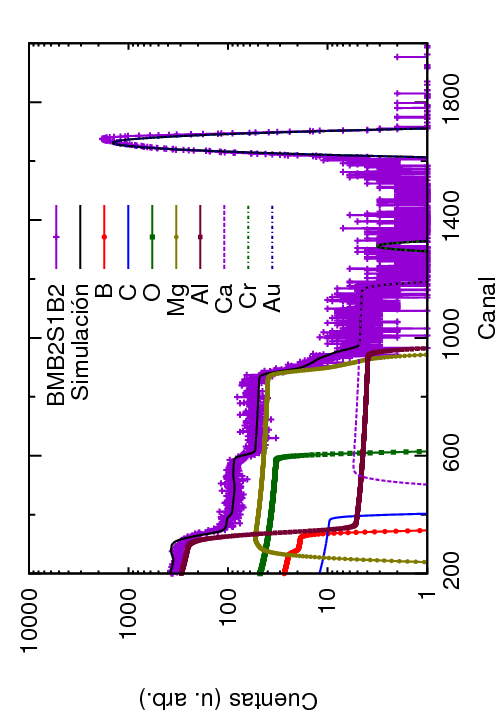
\includegraphics[width=0.58\textwidth, angle=-90]{RBS}
   \end{center}
   \caption[Espectro RBS típico observado para las muestras estudiadas.]{Espectro RBS típico observado para las muestras estudiadas. El espectro que se observa corresponde a la muestra BMB2S1B2. La presencia de Au y Cr se puede explicar teniendo en cuenta que sobre la muestra se evaporaron contactos para medir propiedades de transporte, y el Al y O corresponden al sustrato de zafiro.}
   \label{fig:RBS}
 \end{figure}

 En la Fig. \ref{fig:RBS} se muestra el espectro RBS típico que se pudo observar en las muestras estudiadas. Como puede verse, el método permite observar el Mg y el B presente en la muestra, así como el Al y el O presentes en el sustrato de zafiro (fórmula química Al$_2$O$_{3}$). También se observan impurezas de C y Ca y rastros de Au y Cr debidos a contactos que se evaporaron sobre la muestra para medir propiedades de transporte. En la tabla \ref{tab:composicionRBS} se encuentran resumidos los resultados obtenidos del cálculo de la composición B/Mg para las diferentes muestras estudiadas por medio de la téc\-ni\-ca RBS.

 \begin{table}[h!]
  \centering
  \begin{tabular}{|c|c|c|c|}\hline
	Muestra	& Potencia/W & p/mTorr & Proporción B/Mg\ \\ \hline
	BMB2S1B2 & 50 & 10 & 3,62 \\
	BMB2S3B3 & 100 & 10 & 4,49 \\
	BMB2S4B3 & 50 & 50 &  2,38 \\ \hline
  \end{tabular}
  \caption[Proporción B/Mg para las muestras estudiadas por medio de la técnica RBS.]{Proporción B/Mg para las muestras estudiadas por medio de la técnica RBS. Se muestran además los parámetros de crecimiento que cambiaron entre las diferentes muestras. En todos los casos la temperatura de crecimiento era 225\,$^{\circ}$C y la distancia era 2,75. Las mediciones y el análisis de los datos fueron realizados por los Dres. S. Suárez y L. M. Rodriguez.}
  \label{tab:composicionRBS}
\end{table}

Si se comparan las tablas \ref{tab:depositos} y \ref{tab:composicionRBS} el primer punto llamativo es que se tiene una misma muestra (la BMB2S3B3) que presenta diferentes composiciones para cada técnica, incluso más allá del error de ambos métodos, lo que no es del todo sorprendente si se tienen en cuenta las diferencias que existen entre los métodos utilizados para hacer la estimación. En el caso de la técnica EDX cabe tener en cuenta que se intentó estimar la composición del B, un elemento que se encuentra en el límite de confianza de la técnica, por lo que las conclusiones que se pueden sacar del análisis EDX son más bien cualitativas que cuantitativas. En el caso del estudio por RBS, aunque es una técnica con más sensibilidad al B que el EDX, cabe mencionar que, como se observa en la Fig. \ref{fig:RBS}, el espectro que se espera del boro ocurre a bajas energías, donde la resolución del detector utilizado para hacer el estudio RBS es más pobre.
\newpage
Teniendo en cuenta las imprecisiones observadas en los métodos utilizados para determinar la estequiometría y estructura cristalina de los films crecidos, se decidió completar la caracterización de los films crecidos con mediciones de magnetización y transporte. Este tipo de mediciones, que se encuentran detalladas en la sección siguiente, permitió obtener una descripción completa de las propiedades de los films crecidos.
\subsection{Caracterización de las propiedades magnéticas y de transporte}\label{SS:sptucarac}
Como se explicó al principio del capítulo, la estequiometría de un film y la estructura cristalina formada en el mismo son dos cosas diferentes. Es decir, es posible que se hayan formado granos de MgB$_2$ desconectados entre si, y que en el resto del material exista un exceso de B, lo que explicaría la estequiometría observada, y aún así daría una señal en el SQUID. También es posible que se haya formado un camino de MgB$_2$ con un área muy pequeña, lo que daría una señal imperceptible en el SQUID pero sería observable en una medición de transporte. De ahí que mediciones de magnetización en conjunto con mediciones de transporte permiten determinar completamente si se ha podido formar el superconductor MgB$_2$ en alguno de los films crecidos.
 \begin{figure}[tbh!]
   \begin{center}
	 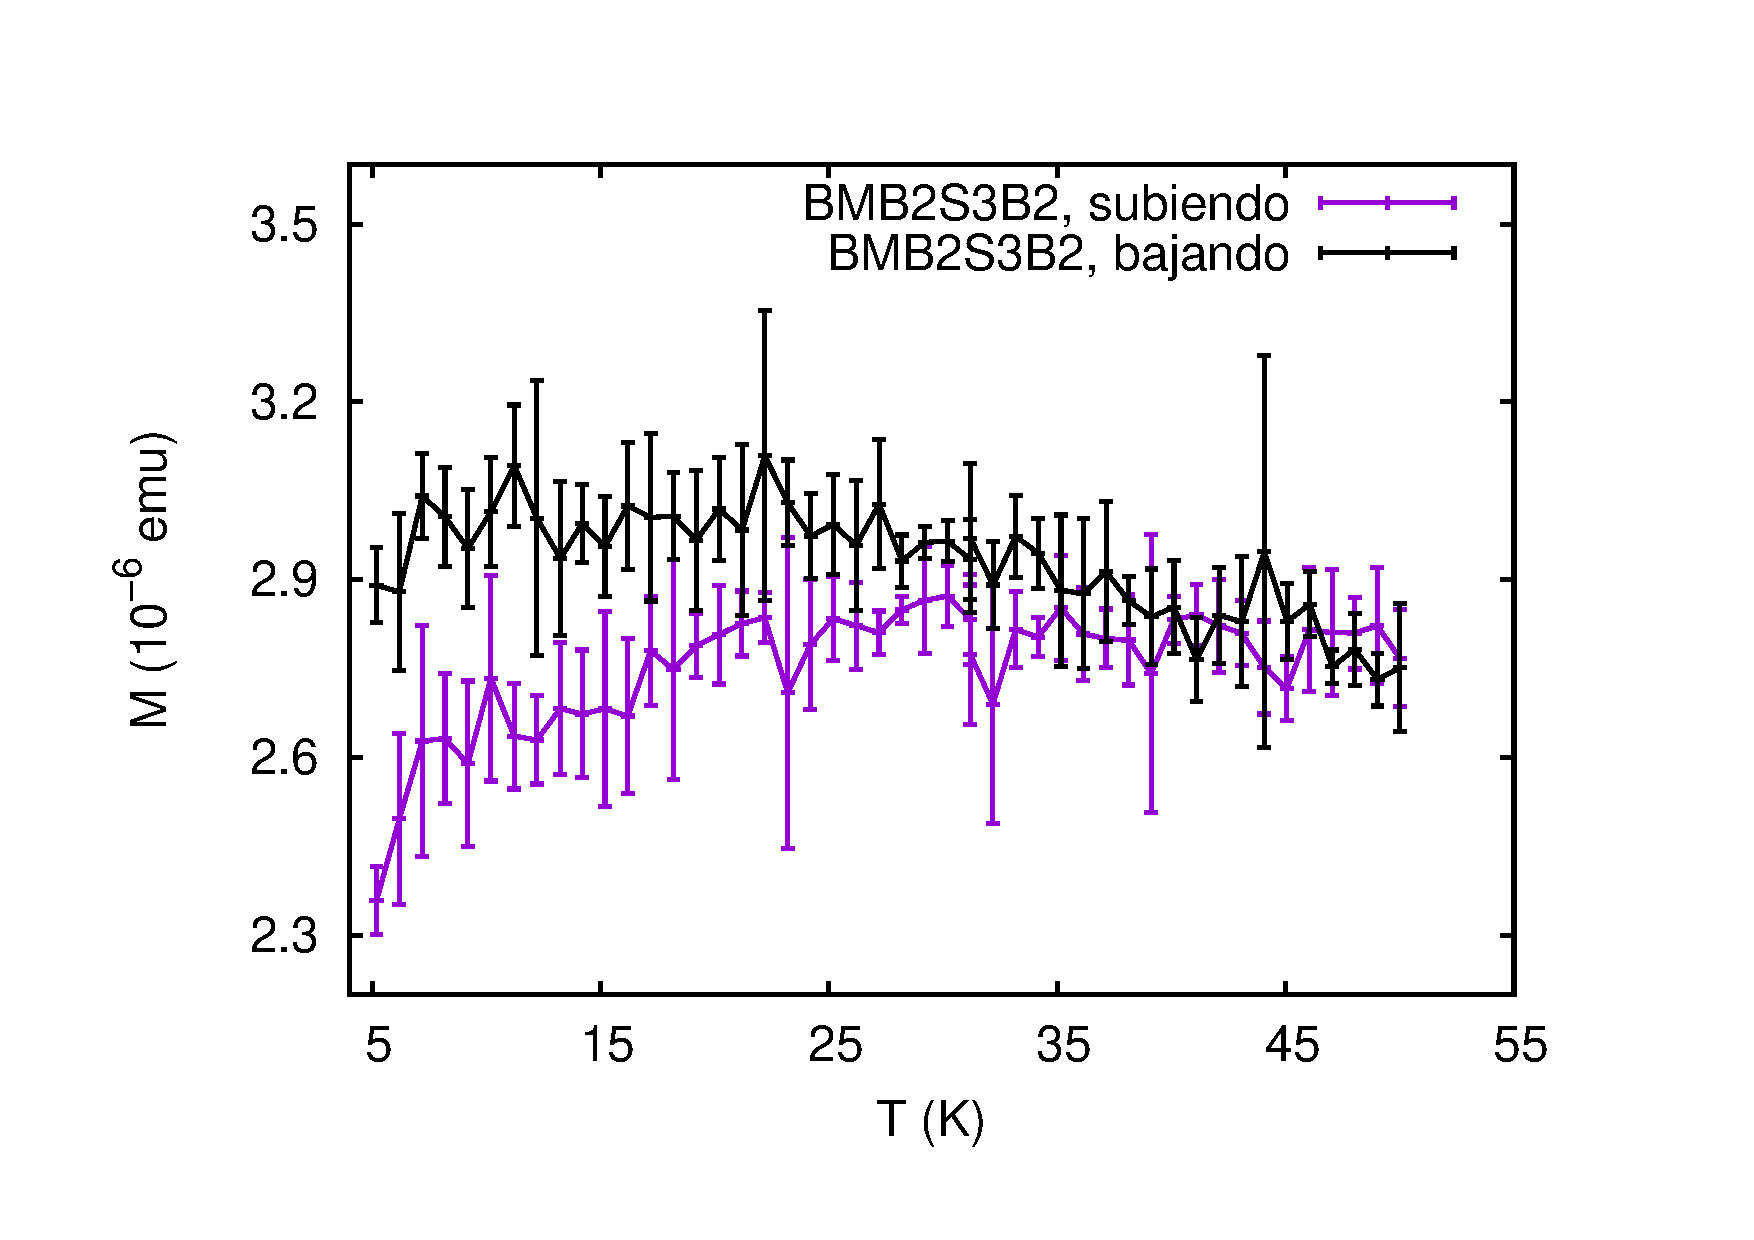
\includegraphics[width=0.9\textwidth, angle=0]{BMB2S4B2_MvsT}
   \end{center}
   \caption[Magnetización en función de la temperatura para la muestra BMB2S3B2, después de realizar un recocido con una pastilla de Mg puro.]{Magnetización en función de la temperatura para la muestra BMB2S3B2, después de realizar un recocido con una pastilla de Mg puro. La aparente irreversibilidad observada se encuentra dentro de límite de resolución del instrumento y no es una prueba confiable de la existencia de superconductividad. A partir de esto se concluyó que los films crecidos por sputtering no resultaron ser superconductores, ni siquiera luego del proceso de recocido. El fallo del recocido se debió probablemente a que el mismo ocurrió a una temperatura demasiado baja.}
   \label{fig:mvst}
 \end{figure}
\newpage
 Dentro de los films depositados por sputtering pudo distinguirse que, al incrementarse la presión de Ar en la cámara durante el crecimiento, los mismos pasaban de ser trans\-pa\-ren\-tes a ser de un color marrón claro. Los primeros eran completamente aislantes mientras que los segundos tenían una resistencia del orden de los k$\Omega$, que es el orden de magnitud de resistencia esperable para un film. Sin embargo, ninguno mostró algún tipo de señal en el SQUID o en mediciones de transporte, probablemente debido a la falta de Mg en los films. Teniendo en cuenta esto se decidió recocer los films crecidos por sputtering junto con una pastilla de Mg puro (pureza 99,5 \%), con el fin de compensar el exceso de boro en las muestras. Se decidió intentar con Mg, y no con MgB$_2$, para reducir la temperatura del recocido. Esto se podía lograr con Mg ya que el mismo tiene un punto de fusión menor que el MgB$_2$, y lo que permite lograr una mayor presión parcial de Mg a una temperatura inferior. Como no existen fases estables de Mg-B  con exceso de Mg, el único compuesto que se debería formar en un proceso de este estilo es el MgB$_2$. Teniendo en cuenta esto se realizaron recocidos de alrededor de 20 hs. de los films crecidos con Mg siguiendo el mismo procedimiento que el utilizado en el capítulo \ref{C:evap}, bajando la temperatura de recocido a 630\,$^{\circ}$C.
 \begin{figure}[tbh!]
   \begin{center}
	 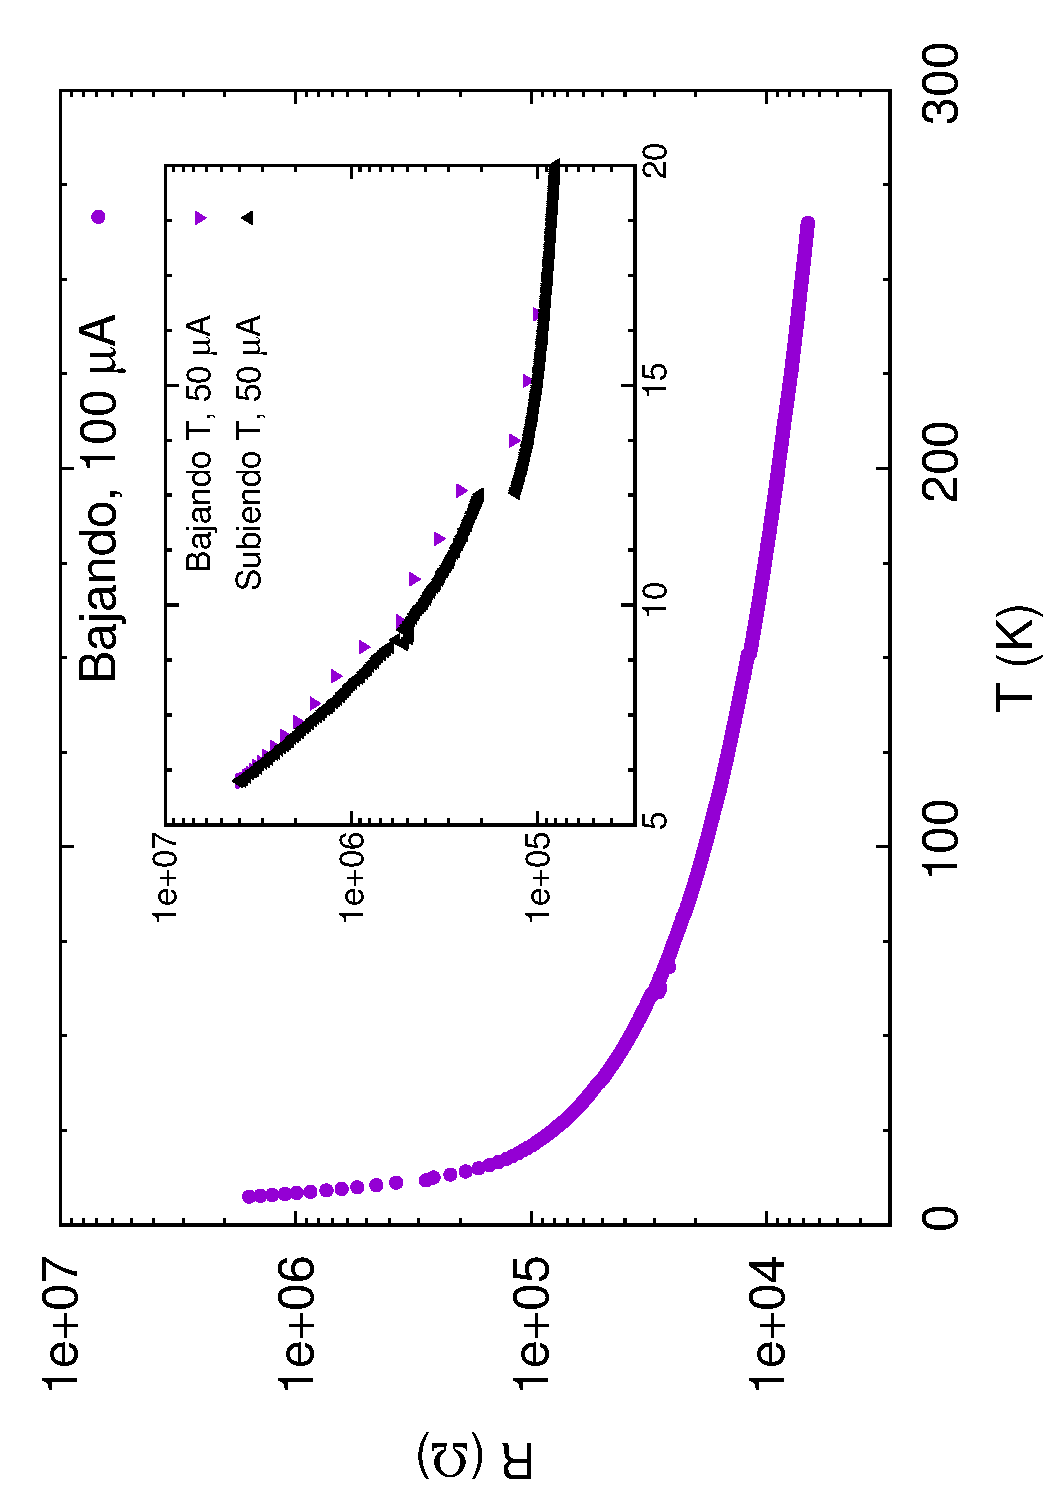
\includegraphics[width=0.55\textwidth, angle=-90]{Rvst_BMB2S1B1}
   \end{center}
   \caption[Medición de la resistencia en función de la temperatura para la muestra BMB2S1B1, luego de ser recocida.]{Medición de la resistencia en función de la temperatura para la muestra BMB2S1B1, luego de ser recocida. El recocido llevó a que las muestras pasasen de ser transparentes y aislantes a tener un color negruzco y una resistencia de algunos k$\Omega$. Puede observarse, sin embargo que la muestra tiene un comportamiento semiconductor en vez de metálico, que es lo que se esperaría si el film fuera de MgB$_2$. A parir de esto se elaboró la conclusión que las películas delgadas no incorporaron la cantidad suficiente de Mg durante el recocido. El salto en resistividad observado a alrededor de 12\,K se debe a un problema con los contactos.}
   \label{fig:rvstS1B1}
 \end{figure}
 
 Luego de extraer a las muestras del recocido se notó que las muestras que eran transparentes adquirieron un color negruzco y pasaron de ser completamente aislantes a tener una resistencia de algunos k$\Omega$. Las muestras que eran marrones se volvieron algo más oscuras pero aparte de eso no mostraron cambios perceptibles en sus propiedades. Se volvió a medir la magnetización en las muestras recocidas, sin embargo, los resultados de las mediciones de magnetización, que se ven la Fig. \ref{fig:mvst}, dieron los mismos resultados que con las muestras antes del recocido. Si bien puede observarse cierta irreversibilidad en la magnetización, el valor de la misma se encuentra cerca del límite de resolución del instrumento. Como se dijo previamente, este comportamiento se observó sistemáticamente en todos los films crecidos, antes y después del recocido.

%\subsection{Caracterización de las propiedades de transporte}\label{SS:Rvst}
%\newpage
 También se procedió a caracterizar las propiedades de transporte de los films recocidos, mostrándose en la Fig. \ref{fig:rvstS1B1} los resultados obtenidos para la muestra BMB2S1B1, donde se puede apreciar que el comportamiento de la resistencia del film al disminuir la temperatura se asemeja más al de un semiconductor que al del MgB$_2$. El salto observado a $T \ \approx \  12$\,K es debido a problemas con los contactos colocados sobre la muestra. La conclusión que puede extraerse tanto de las mediciones de magnetización como de las de transporte es que no se ha podido lograr la fase MgB$_2$, ni siquiera luego del proceso de recocido. El motivo por el que el recocido haya fallado se debe probablemente a que como la temperatura a la que ocurrió el mismo no fue lo suficientemente alta, no se pudo hacer difundir la cantidad suficiente de Mg a través del film como para formar la fase MgB$_2$. A partir de esto resulta claro que si se busca fabricar los films por medio de un proceso de recocido resulta necesario realizarlo utilizando MgB$_2$. De esta forma se puede incrementar la temperatura a la que ocurre el recocido de modo de permitir a los átomos de Mg difundir a través del film. Esta solución trae aparejado el problema de que al aumentar la temperatura, el sustrato va a reaccionar con la muestra depositada en él, por lo que si desea continuar con el proceso de recocido, es preciso buscar un sustrato que reaccione poco o nada con el MgB$_2$ a altas temperaturas.
%\begin{figure}[tbh!]
%  \begin{center}
%	 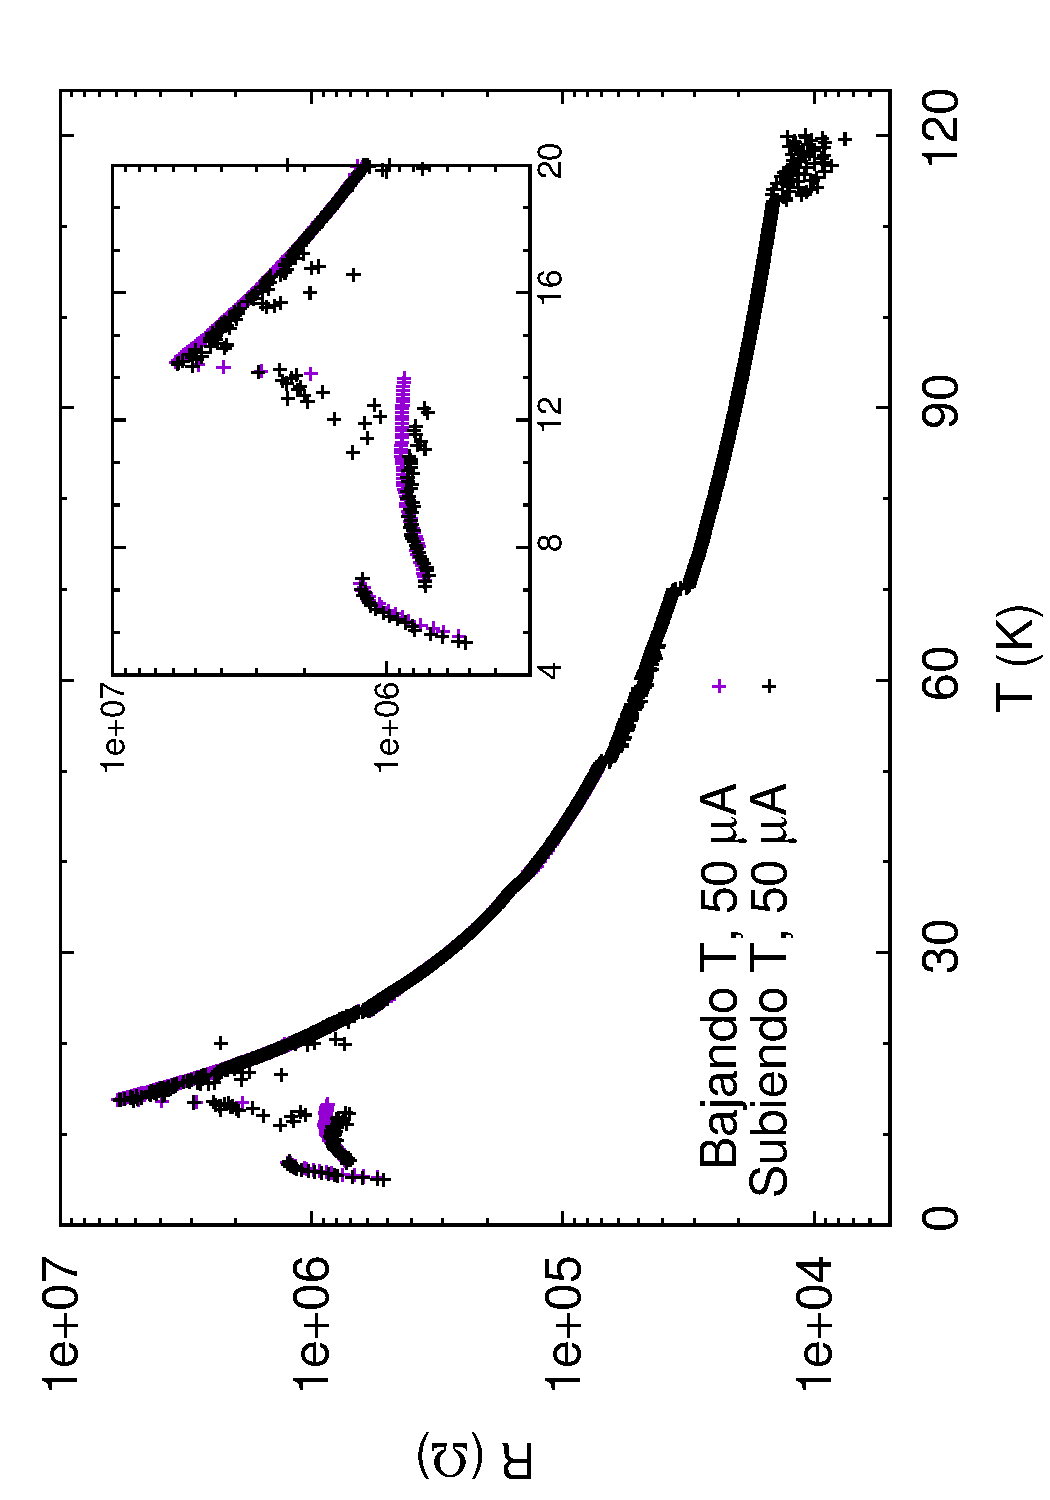
\includegraphics[width=0.55\textwidth, angle=-90]{Rvst_BMB2S2B1}
 %  \end{center}
 %  \caption{Rvst para BMB2S2B1}
 %  \label{fig:rvstS2B1}
 %\end{figure}
\nomenclature{$T_{crec}$}{Temperatura a la que se crece un film.}
\nomenclature{$v_{crec}$}{Velocidad de crecimiento de un film.}
\nomenclature{EDX}{Siglas en inglés para espectroscopia por rayos X característicos.}
\nomenclature{RBS}{Siglas en inglés para retrodispersión de Rutherford.}
\nomenclature{$\varepsilon$}{Constante de proporcionalidad.}
\nomenclature{$x$}{Proporción B/Mg de una muestra.}
\section{Análisis del método}\label{S:sputanalisis}
La técnica de crecimiento por sputtering tiene la ventaja de ser un método altamente reproducible que permite obtener films con una adherencia muy superior a los que se obtienen por evaporación. Sin embargo, las pruebas realizadas hasta ahora parecen indicar que no se puede obtener un film de MgB$_2$ a partir de un blanco del mismo material, debido a que no se logra transferir material del blanco al sustrato manteniendo la proporción B/Mg adecuada. Este problema podría solucionarse realizando una técnica mixta que consistiría en crecer films de Mg y B o de B puro para luego hacer un recocido a altas temperaturas con una pastilla bulk de MgB$_2$, lo que obligaría a buscar un sustrato que no reaccione con el film durante con el recocido, ya que de otra forma resulta poco probable que los films obtenidos sean útiles para la fabricación de un detector de neutrones. La otra alternativa es depositar en forma independiente y simultánea B y Mg, lo que permitiría controlar mejor la cantidad de material de cada elemento que se deposita en el sustrato. Con esto se debería lograr un film de MgB$_2$ que tenga las propiedades requeridas para la construcción del detector evitando el paso del recocido.
